\documentclass[11pt,letterpaper]{article}
\PassOptionsToPackage{hyphens}{url}
\usepackage[margin=.83in,top=.8in,bottom=.8in,headheight=15pt]{geometry}
\usepackage[T1]{fontenc}
\usepackage{lmodern,amsmath,amssymb,mathtools,bm,booktabs,array,graphicx,tikz}
\usetikzlibrary{arrows.meta,positioning,calc,decorations.pathreplacing,patterns}
\definecolor{ink}{HTML}{17344D}\definecolor{accent}{HTML}{087E8B}\definecolor{pale}{HTML}{EDF5F5}\definecolor{gold}{HTML}{AD6B19}
\providecommand{\dd}{\,\mathrm{d}}\providecommand{\R}{\mathbb{R}}
\providecommand{\E}{\mathbb{E}}\providecommand{\Var}{\operatorname{Var}}
\providecommand{\Cov}{\operatorname{Cov}}\providecommand{\diag}{\operatorname{diag}}
\providecommand{\norm}[1]{\left\lVert#1\right\rVert}
\providecommand{\abs}[1]{\left|#1\right|}
\usepackage{microtype,hyperref,fancyhdr,enumitem,amsthm,sectsty,needspace}
\allsectionsfont{\raggedright}
\hypersetup{colorlinks=true,linkcolor=ink,urlcolor=accent,pdfauthor={Zan Ahmad},pdftitle={A reduced cardiac reaction--diffusion wave / Lecture notes}}
\setlength{\parindent}{0pt}\setlength{\parskip}{6pt}\linespread{1.07}
\setlist{itemsep=3pt,topsep=4pt,leftmargin=*}
\emergencystretch=2em\clubpenalty=10000\widowpenalty=10000
\pagestyle{fancy}\fancyhf{}\fancyhead[L]{\small Computational Cardiology}\fancyhead[R]{\small Lecture 10}
\fancyfoot[L]{\footnotesize Zan Ahmad}\fancyfoot[R]{\footnotesize\thepage}\renewcommand{\headrulewidth}{.3pt}
\newtheorem{proposition}{Proposition}\newtheorem{theorem}{Theorem}\newtheorem{lemma}{Lemma}
\theoremstyle{definition}\newtheorem{definition}{Definition}\newtheorem{example}{Example}
\numberwithin{equation}{section}
\begin{document}
{\small\scshape Computational Cardiology\hfill Lecture 10}\par\medskip
{\raggedright\hyphenpenalty=10000\exhyphenpenalty=10000\LARGE\bfseries\color{ink} A reduced cardiac reaction--diffusion wave\par}\medskip
{\small Lecture notes}\par\bigskip
The Mitchell--Schaeffer model combines a nonlinear inward term, linear recovery current and a threshold-dependent gate. Adding shared-face diffusion produces a homogeneous strand model. An admissible numerical step follows from explicit inequalities, while measured propagation speed requires a separate definition of stimulus, sensors and arrival time.

\section{The scaled cardiac reaction system}
\hypertarget{note-the-scaled-cardiac-reaction-system}{}\label{note:the-scaled-cardiac-reaction-system}
{\small \href{slides.html\#frame=a-scaled-cardiac-reaction-system\&step=1}{Slides for this section} \quad \href{../modules/animations/excitable-wave.html}{Excitation and propagation}}\par
We now change from the neuronal HH cell to the reduced cardiac model of Mitchell and Schaeffer. Its variables are scaled voltage v and a recovery gate h, both dimensionless. This h is not automatically the sodium-inactivation gate from the previous lesson: the symbols belong to different equations and interpretations. The model combines a nonlinear aggregate inward term with a linear outward term. It can support a cardiac-like excitation and recovery pattern without resolving individual ionic currents or calcium concentrations.

The reaction equation uses inward contribution h v\ensuremath{^{2}}(1\ensuremath{-}v)/tau\_in and outward contribution v/tau\_out. The recovery gate opens toward one below a voltage threshold and closes toward zero above it. We use tau\_in=0.3, tau\_out=6, tau\_open=120 and tau\_close=150 milliseconds, with threshold v\_gate=0.13, from the primary paper's illustrative parameter set. Equality at the threshold uses the closing branch in this implementation. That convention must be declared because the piecewise equation otherwise leaves equality ambiguous.

The stimulus has units of scaled voltage per millisecond, not microamperes per square centimetre. A conversion to a physical voltage or current density would require an additional stated scaling and capacitance. Accordingly, our plots retain dimensionless voltage axes. These equations supply a compact reaction mechanism for a reduced tissue calculation, not a validated prediction for an individual heart.

\[
\partial_t v=\frac{hv^2(1-v)}{\tau_{\rm in}}-\frac{v}{\tau_{\rm out}}+I_{\rm stim}+D\partial_{xx}v
\]
v and h are dimensionless; time ms; position cm; D in cm\ensuremath{^{2}}/ms; stimulus in ms\ensuremath{^{-1}}.

\[
\partial_t h=\begin{cases}(1-h)/\tau_{\rm open},&v<v_{\rm gate},\\-h/\tau_{\rm close},&v\ge v_{\rm gate}.\end{cases}
\]
The equality convention is explicit in the new implementation.

The equilibrium $(v,h)=(0,1)$ is preserved in the absence of stimulus: the voltage reaction vanishes and the low-voltage gate branch has zero derivative. The parameter values define relaxation times, not directly measured ionic conductances. Converting scaled voltage to mV would require a declared affine voltage scale, and converting the source to current density would additionally require capacitance.
\section{Conservative coupling on a sealed strand}
\hypertarget{note-conservative-coupling-on-a-sealed-strand}{}\label{note:conservative-coupling-on-a-sealed-strand}
{\small \href{slides.html\#frame=shared-diffusive-face-fluxes\&step=1}{Slides for this section} \quad \href{../modules/animations/excitable-wave.html}{Excitation and propagation}}\par
Consider a sealed one-dimensional strand of length two centimetres with constant diffusion coefficient 0.001 cm\ensuremath{^{2}}/ms. A cell-centred grid divides it into equal control volumes. Integrating the diffusion equation over one cell gives its voltage-average rate as left incoming flux minus right outgoing flux, divided by cell width. For constant D, each interior face uses the difference between neighboring voltages divided by their centre separation. The same face flux appears with opposite signs in the two adjacent balances.

At a sealed end the normal diffusive flux is zero. The boundary cell therefore has one neighbor contribution instead of two. Summing all diffusion-only cell balances cancels every interior face and leaves zero boundary contribution, so the spatial integral of scaled voltage is conserved during that substep. This is a numerical identity for passive diffusion under these boundary conditions. Reaction and stimulus generally change that integral, so demanding conservation over a full excited trajectory would test the wrong property.

This homogeneous strand omits anisotropy, changing cross-sectional area, branching and extracellular current. A neuronal cable tree needs membrane areas, axial conductances and branch-current conservation derived from its geometry; one cannot transplant this equal-width cardiac stencil and claim to have represented the tree. Those distinctions matter even when both models contain a term informally called diffusion.

\[
\frac{d v_i}{dt}=\frac{F_{i-1/2}-F_{i+1/2}}{\Delta x},\quad F_{i+1/2}=-D\frac{v_{i+1}-v_i}{\Delta x}
\]
Flux F has units cm/ms for dimensionless voltage; this is a scaled diffusive flux, not a reported electrical current.

Let $L_h$ denote the nonnegative graph Laplacian of the sealed cell chain, including the factor $D/\Delta x^2$. Then the diffusion equation is $\dot v=-L_hv$, with
\[
 L_h\boldsymbol1=0,\qquad
 v^{\mathsf T}L_hv=\frac D{\Delta x^2}\sum_{i=1}^{N-1}(v_{i+1}-v_i)^2\ge0.
\]
Thus diffusion preserves the sum and decreases the squared norm. Reaction and stimulus need not preserve either quantity.

\paragraph{Calculation.} For three cells with values 0.2, 0.8 and 0.4, dx=0.1 cm and D=0.001 cm\ensuremath{^{2}}/ms, calculate the diffusion-only slopes with sealed ends.

D/dx\ensuremath{^{2}}=0.1 ms\ensuremath{^{-1}}. The first slope is 0.1(0.8\ensuremath{-}0.2)=0.06 ms\ensuremath{^{-1}}.

The middle slope is 0.1(0.2\ensuremath{-}2\ensuremath{\times}0.8+0.4)=\ensuremath{-}0.10 ms\ensuremath{^{-1}}.

The last slope is 0.1(0.8\ensuremath{-}0.4)=0.04 ms\ensuremath{^{-1}}. Multiplying their sum by dx gives zero.

Diffusion redistributes the field while preserving its discrete integral.
\Needspace{10\baselineskip}
\section{Gate, reaction and diffusion substeps}
\hypertarget{note-gate-reaction-and-diffusion-substeps}{}\label{note:gate-reaction-and-diffusion-substeps}
{\small \href{slides.html\#frame=exact-frozen-branch-gate-evolution\&step=1}{Slides for this section} \quad \href{../modules/animations/excitable-wave.html}{Excitation and propagation}}\par
The new solver separates reaction from diffusion. First it advances the gate exactly while freezing the old voltage's threshold branch. It then freezes the quadratic activation factor using the old voltage and the updated gate, but treats the remaining linear voltage factors implicitly. If a denotes h\_new times v\_old squared divided by tau\_in, the resulting reaction value is [v\_old+dt(a+stimulus)] divided by [1+dt(a+1/tau\_out)]. This formula is an original first-order teaching discretization, not a solver copied from the primary paper.

For old voltage between zero and one, nonnegative a, and stimulus between zero and 1/tau\_out, the numerator is nonnegative and does not exceed the denominator. Thus the reaction step preserves the interval. The exact gate update also preserves its interval. Backward-Euler diffusion solves a tridiagonal system with positive diagonal, nonpositive neighbor coefficients and unit row sums; this preserves constants and the bounded range. The code checks finite values and rejects inadmissible states rather than silently clipping them.

These structural properties are valuable but do not remove time error. Freezing the reaction coefficient and splitting the operators gives a first-order coupled method. The sharp gate switch adds another source of sensitivity near threshold. We therefore test a smooth, spatially uniform reaction case against DOP853 separately from the active wave. We also test the diffusion solver against the exact backward-Euler amplification of a discrete cosine mode, so a correct reaction test cannot conceal an incorrect spatial matrix.

\[
v^*=\frac{v^n+\Delta t(a+I)}{1+\Delta t(a+1/\tau_{\rm out})},\quad a=\frac{h^{n+1}(v^n)^2}{\tau_{\rm in}}
\]
This bound argument assumes 0\ensuremath{\le}v\_old,h\_new\ensuremath{\le}1 and 0\ensuremath{\le}I\ensuremath{\le}1/tau\_out. Diffusion follows the reaction update.

To prove the reaction bound, subtract its numerator from its denominator:
\[
 1+\Delta t(a+1/\tau_{out})-
 [v^n+\Delta t(a+I)]
 =1-v^n+\Delta t(1/\tau_{out}-I)\ge0.
\]
The argument requires $0\le I\le1/\tau_{out}$. Backward-Euler diffusion gives $(I+\Delta tL_h)v^{n+1}=v^*$. Its inverse is nonnegative and its rows sum to one, so it also maps $[0,1]^N$ into itself. These statements concern bounds, not the accuracy of front location.
\section{A fixed physical stimulus and sensor geometry}
\hypertarget{note-a-fixed-physical-stimulus-and-sensor-geometry}{}\label{note:a-fixed-physical-stimulus-and-sensor-geometry}
{\small \href{slides.html\#frame=a-fixed-spatial-source-panel-1\&step=1}{Slides for this section} \quad \href{../modules/animations/excitable-wave.html}{Excitation and propagation}}\par
A mesh comparison is meaningful only if it represents the same experiment. The initial state is v=0, h=1. A stimulus of 0.1 per millisecond starts at one millisecond, lasts two milliseconds and occupies the first 0.1 centimetre. If a stimulus edge cuts through a cell, that cell receives the fraction of its width that overlaps the stimulated region. This preserves the integrated source under refinement instead of assigning an arbitrary whole-cell block on each mesh.

The timeline includes pulse onset and offset exactly. The integrated source is amplitude times duration times stimulated width, here 0.02 centimetre in scaled-voltage integral units. This quantity is not an electrical charge in microcoulombs: the model has not supplied that physical conversion. It is nevertheless a useful consistency check that the same forcing was applied to different grids and time steps.

We measure at positions 0.6 and 1.2 centimetres, using linear interpolation between cell centres rather than choosing the nearest grid index. Arrival means the first upward crossing of scaled voltage 0.5. Interpolating between the two surrounding time samples estimates that crossing more precisely than recording the next stored sample. If a sensor never crosses, arrival is missing, not zero. Simultaneous or reversed arrivals also do not define a positive forward conduction speed for this two-sensor measurement.

For a stimulus interval $[0,\ell_s]$, cell $K_i$ receives the fractional overlap
\[
 I_i(t)=I_0(t)\frac{|K_i\cap[0,\ell_s]|}{\Delta x}.
\]
Summing $\Delta x I_i$ recovers $I_0\ell_s$ even when the stimulus endpoint cuts a cell. Splitting time intervals at pulse edges likewise preserves the prescribed integrated source.
\begin{center}\begin{minipage}{.98\linewidth}\centering
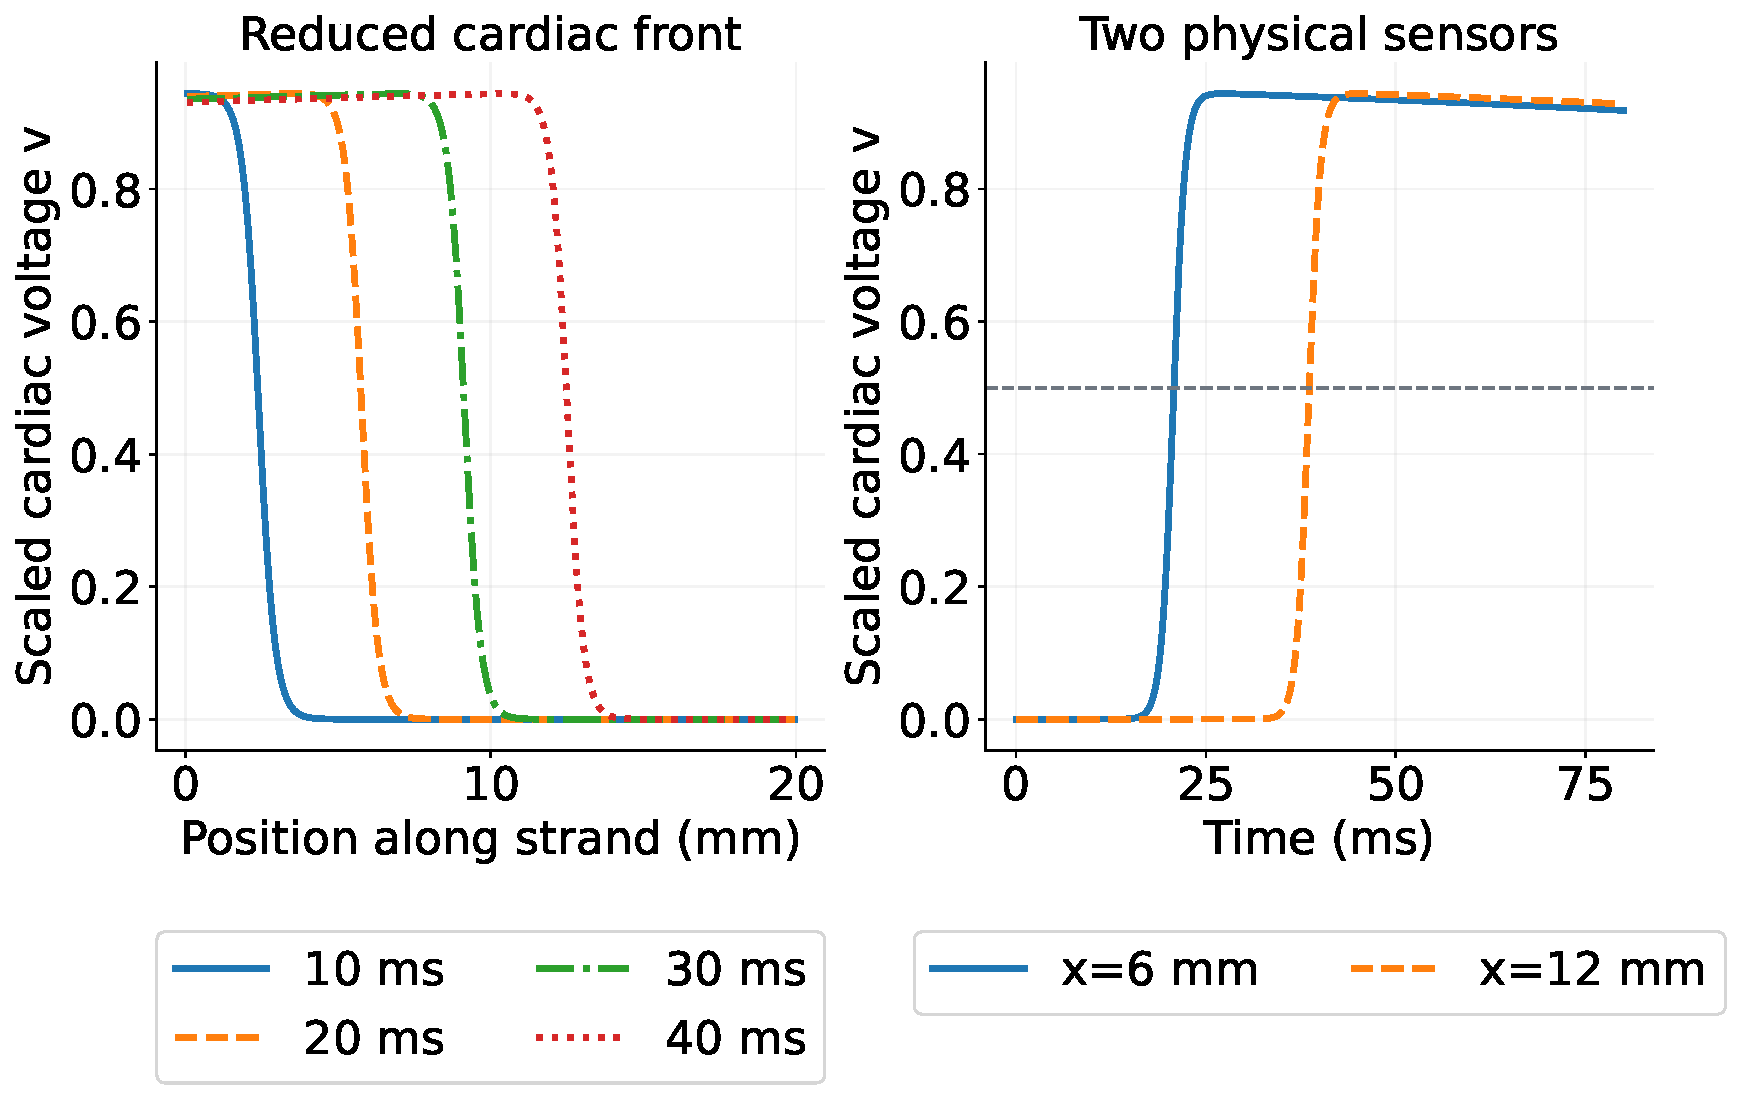
\includegraphics[width=.96\linewidth,height=.57\textheight,keepaspectratio]{cardiac-wave.pdf}\par\smallskip
{\small Original homogeneous one-dimensional reduced cardiac computation: 20 mm sealed strand, D=\allowbreak{}0.001 cm$^2$/ms, 200 cells and nominal dt=\allowbreak{}0.02 ms. Voltage is scaled and dimensionless; the dashed sensor level is 0.5.}
\end{minipage}\end{center}
\section{Threshold arrival and conduction speed}
\hypertarget{note-threshold-arrival-and-conduction-speed}{}\label{note:threshold-arrival-and-conduction-speed}
{\small \href{slides.html\#frame=interpolate-an-upward-crossing\&step=1}{Slides for this section} \quad \href{../modules/animations/excitable-wave.html}{Excitation and propagation}}\par
With a specified arrival criterion, speed is the distance between sensors divided by their arrival-time difference. The default calculation gives arrivals near 20.778 and 38.605 ms at six and twelve millimetres. Their delay is about 17.827 ms, so the measured speed is approximately 0.337 m/s. This is a result of the stated reduced model, stimulus and numerical resolution. A single plausible-looking speed is not evidence of a physiological calibration.

Arrival-time estimation interpolates a crossing on one time interval. If the lower and upper samples are y0 and y1 at times t0 and t1, the fraction of the interval is (threshold\ensuremath{-}y0)/(y1\ensuremath{-}y0). This formula assumes an upward crossing with unequal endpoint values. The interpolation formula defines the measurement operation separately from the reaction--diffusion solve.

Different thresholds can yield different arrival estimates because a wavefront has finite width and may change shape. Near a stimulus site, the waveform may still be forming. Near a sealed endpoint, reflected or boundary-influenced behavior can also matter. Record sensor positions, threshold, mesh, step and propagation direction with the result. Our display ends at eighty milliseconds and emphasizes the front; it should not be described as a complete action-potential-duration study.

\[
t_*=t_0+\frac{v_*-v_0}{v_1-v_0}(t_1-t_0),\quad c=\frac{x_2-x_1}{t_{*,2}-t_{*,1}}
\]
One cm/ms equals 10 m/s. Use only a valid upward bracket and positive forward delay.

For sensor separation $\Delta x_s$ and delay $\Delta t_s$, perturbing the arrival estimates gives
\[
 \frac{\delta c}{c}\simeq\frac{\delta\Delta x_s}{\Delta x_s}
 -\frac{\delta\Delta t_s}{\Delta t_s}.
\]
A short delay magnifies a fixed absolute timing error. The threshold and sensor placement are therefore part of the observable, rather than incidental plotting choices.
\section{Component analysis and coupled refinement}
\hypertarget{note-component-analysis-and-coupled-refinement}{}\label{note:component-analysis-and-coupled-refinement}
{\small \href{slides.html\#frame=timing-error-propagates-into-speed-panel-1\&step=1}{Slides for this section} \quad \href{../modules/animations/excitable-wave.html}{Excitation and propagation}}\par
We separate three questions. First, does the implementation satisfy its own algebraic properties? Tests preserve the resting state, keep gates bounded, conserve the diffusion-only integral and prevent remote excitation when coupling is removed. Second, does the discretization approach the intended equations? A passive sealed cosine has a known continuous decay rate. Comparing exact semi-discrete decay with that continuous solution isolates spatial error and gives approximately second-order convergence for this smooth field. A separate uniform reaction test approaches first order in time.

Third, how sensitive is the actual measured wave speed? We compare 100, 200 and 400 cells at a fixed small step, then four steps at 400 cells. Both sequences show decreasing successive differences in this fixture. They do not provide an exact wave-speed solution or prove a universal order for threshold-crossing observables. Spatial and temporal errors can interact, so varying both together without a plan would obscure which error is changing.

Biological validation would require relevant experimental observables, parameter justification and a comparison appropriate to the intended tissue. More complex geometry, anisotropic conductivity, bidomain coupling and detailed ionic models define more elaborate models. They introduce new equations and evidence requirements rather than automatically improving the credibility of this small calculation.

For passive sealed diffusion, a cosine mode has continuous decay rate $D(k\pi/L)^2$ and the cell-centered discrete mode has rate
\[
 \lambda_{k,h}=\frac{4D}{\Delta x^2}\sin^2\!\left(\frac{k\pi}{2N}\right).
\]
The discrete rate differs by $O(\Delta x^2)$ for a fixed smooth mode. This spatial statement and first-order reaction splitting do not automatically assign one convergence order to a threshold-crossing speed in the nonlinear wave.
\begin{center}\begin{minipage}{.98\linewidth}\centering
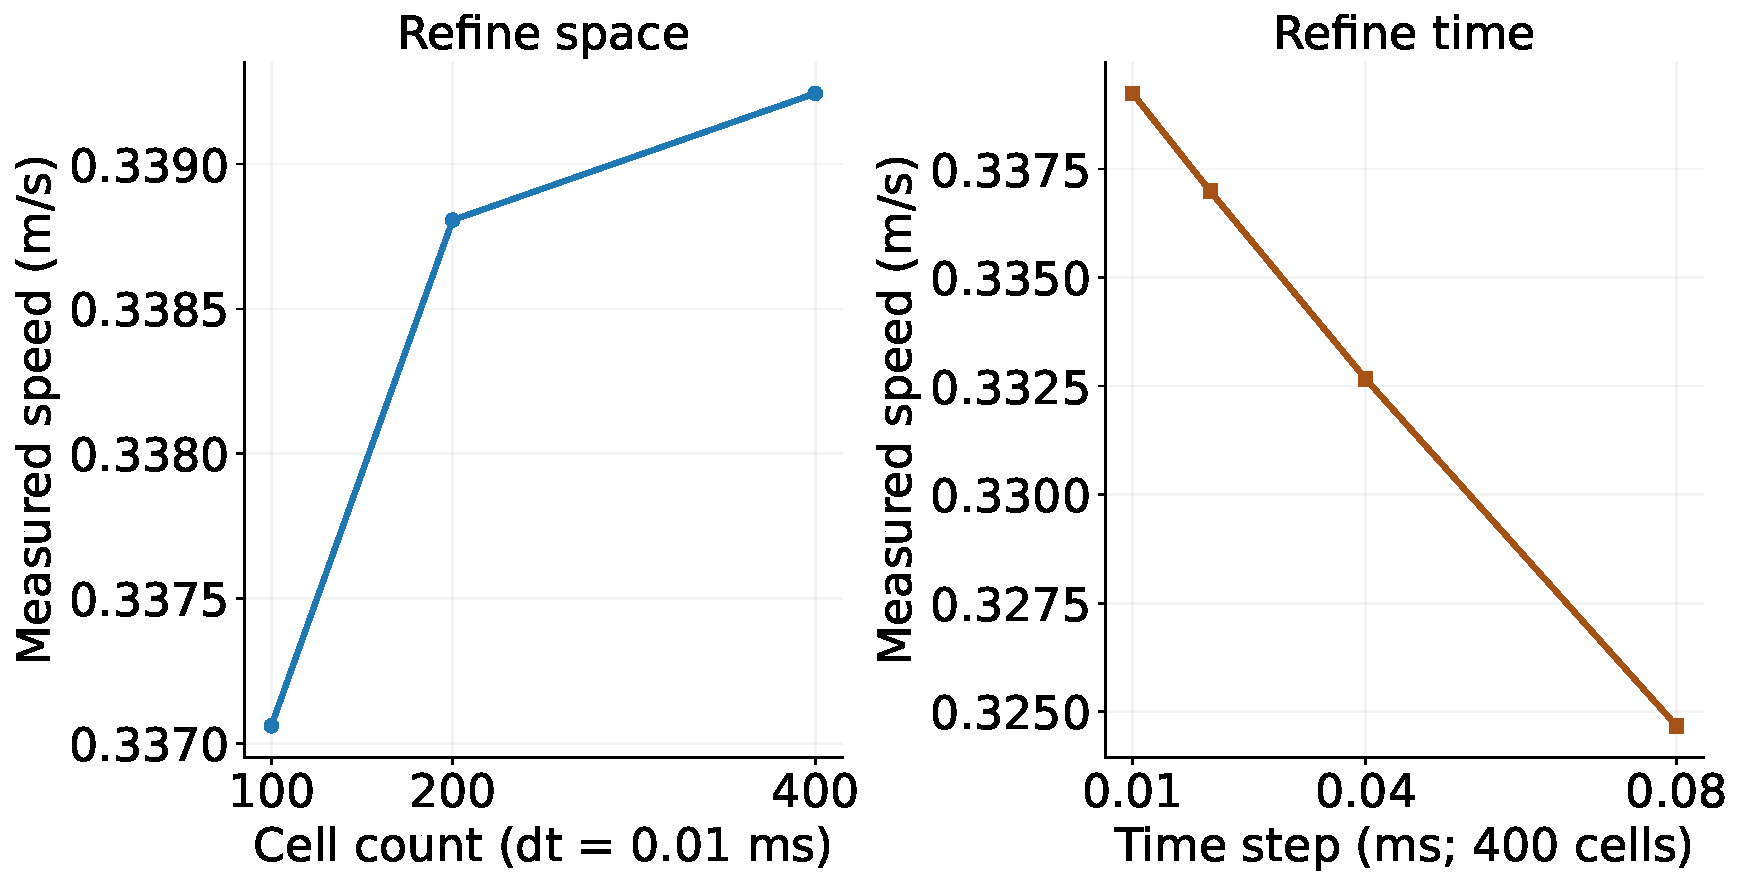
\includegraphics[width=.96\linewidth,height=.57\textheight,keepaspectratio]{wave-refinement.pdf}\par\smallskip
{\small Original speed comparisons keep the physical stimulus and sensors fixed. Spatial refinement uses dt=\allowbreak{}0.01 ms; temporal refinement uses 400 cells. Decreasing differences support numerical consistency for this fixture without claiming an exact physiological speed.}
\end{minipage}\end{center}
\bigskip
\section*{Exercises}
\par\noindent\begin{minipage}{\linewidth}
\subsection*{E1. Derive a sealed diffusion budget}
Use three equal cells, dx=\allowbreak{}0.2 cm, D=\allowbreak{}0.002 cm$^2$/ms and values [0.1,0.5,0.9].

\textbf{a} Calculate the three diffusion-only derivatives and their weighted sum.

\end{minipage}\par\medskip
\textbf{b} A full simulation's integral increases during stimulation. Is this necessarily a conservation bug?

\par\noindent\begin{minipage}{\linewidth}
\subsection*{E2. Measure an arrival and convert its units}
At the first sensor a trace rises from 0.35 at 12 ms to 0.65 at 13 ms. The second sensor is 0.8 cm farther along and crosses the same 0.5 threshold at 32.5 ms.

\textbf{a} Interpolate the first arrival and calculate forward speed in m/s.

\end{minipage}\par\medskip
\textbf{b} How should the report change if the second sensor never crosses during the recording window?

\par\noindent\begin{minipage}{\linewidth}
\subsection*{E3. Audit fixed forcing across meshes}
The scaled stimulus is 0.08 ms$^-$$^1$ for 3 ms over the first 0.15 cm. A grid has dx=\allowbreak{}0.1 cm.

\textbf{a} Give the source amplitudes in the first two cells and the integrated source over space and time.

\end{minipage}\par\medskip
\textbf{b} Why is this value not automatically an injected charge in microcoulombs?

\par\noindent\begin{minipage}{\linewidth}
\subsection*{E4. Separate structural correctness and accuracy}
A solver keeps 0$\leq$v,h$\leq$1 and conserves the diffusion-only sum, but its measured speed changes substantially when dt is halved.

\textbf{a} Explain why the observations are compatible.

\end{minipage}\par\medskip
\textbf{b} Propose separate component and coupled checks before interpreting a physiological speed.

\section*{References}
\noindent\begin{minipage}{\linewidth}
Zan Ahmad, Advanced Topics in Computational Cardiology syllabus, Fall 2024. PDF pages 1--2.

\end{minipage}\par\medskip
\noindent\begin{minipage}{\linewidth}
Hoppensteadt and Peskin, Modeling and Simulation in Medicine and the Life Sciences, second edition. Printed page 317 / supplied PDF page 327: diffusion bridge; not a source for the specific cardiac reaction model.

\end{minipage}\par\medskip
\noindent\begin{minipage}{\linewidth}
Mitchell and Schaeffer, A Two-Current Model for the Dynamics of Cardiac Membrane (2003). Printed pages 769--772; author-hosted PDF pages 3--6, equations 1--5 and Figure 1 parameters.

\url{https://homepage.divms.uiowa.edu/~mtchll/2Current.pdf}
\end{minipage}\par\medskip
\noindent\begin{minipage}{\linewidth}
Zan Ahmad, Action Potential Propagation in Branched Neuronal Cables. Current 8-page report, sections 2--3, PDF pages 1--3.

\url{https://zanahmad.com/files/AP_Propagation.pdf}
\end{minipage}\par\medskip
\end{document}
